% ----------------------------------------------------------------------

\chapter{\textbf{O protótipo}} % Este comando é utilizado para criar capítulos



\begin{figure}[h!]
	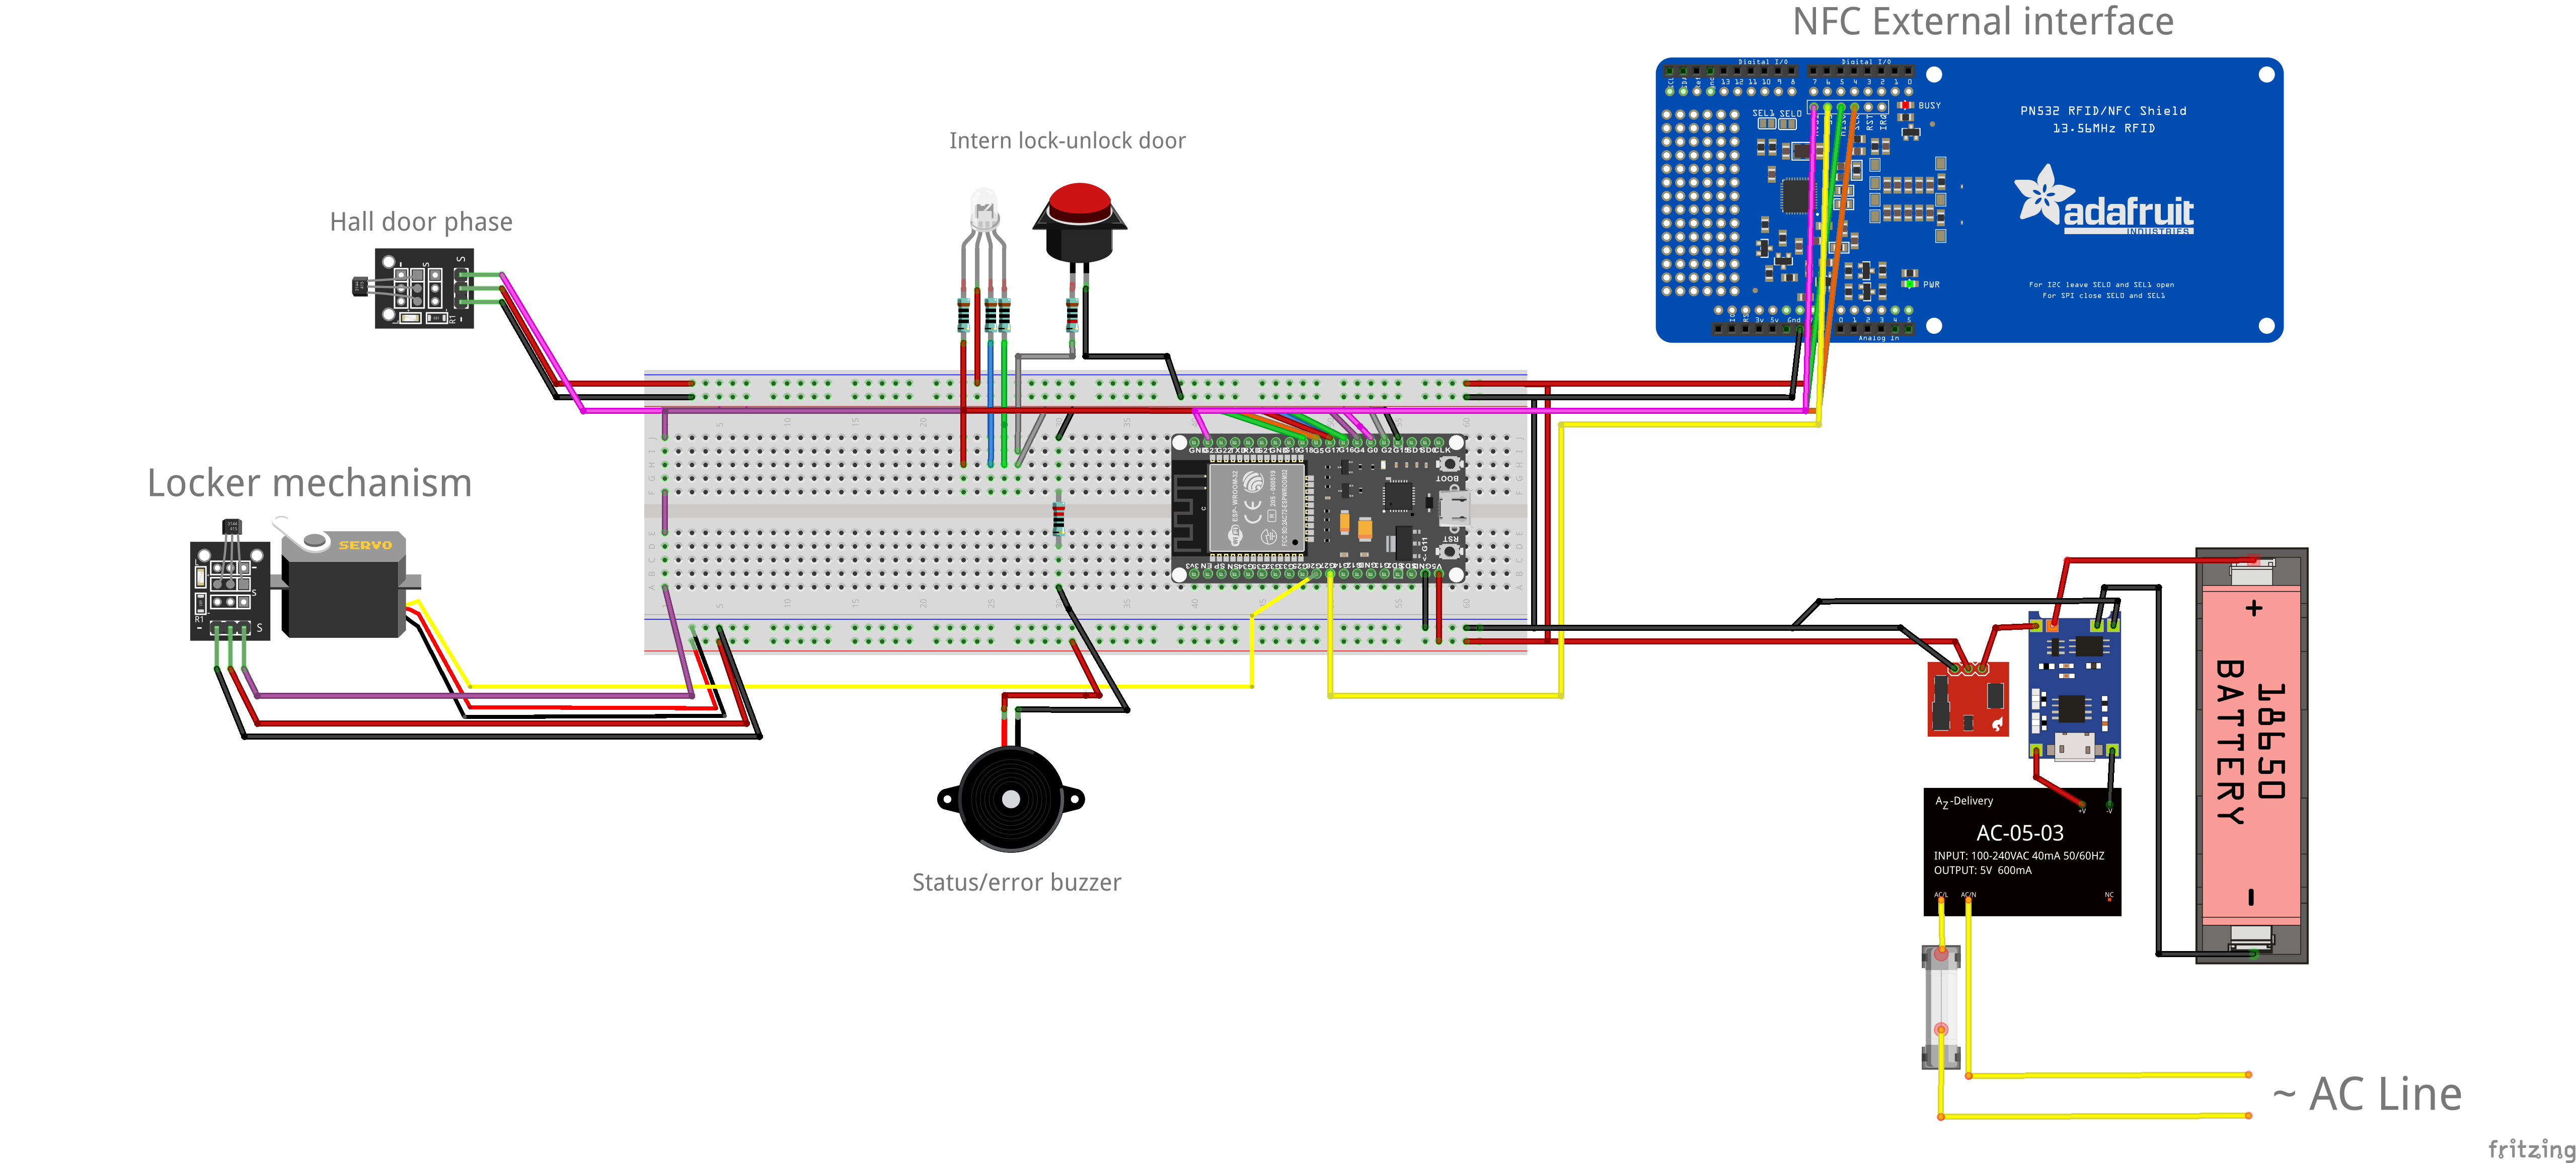
\includegraphics[width=\linewidth]{topics/sketch_bb.png}
	\caption{Diagrama eletronico do protótipo do dispositivo IoT. Fonte: autor}
	\label{fig:dataperformgraph}
\end{figure}

Os dispositivos de Internet das coisas devem se basear numa configuração mínima  ou superior a um microcontrolador ESP32, de baixo custo e proporciona o melhor entre custo benefício para protótipos em dispositivos de Internet das coisas, possui integrado funcionalidades de comunicação em rede Wireless, sendo primordial para os dispositivos a conexão de rede, o processador e memória são compatíveis para o projeto. Os principais pontos são seu espaço extremamente reduzido para a quantidade de funcionalidades presentes.\par
Neste projeto existem algumas formas de integração com o usuário, a primeira é o terminal RFID que proporciona a liberação da fechadura com um controle de acesso por usuário específico, ou seja, somente usuários autorizados previamente na plataforma conseguem destravar o mecanismo. A segunda iteração seria um botão interno para travamento ou liberação do mecanismo, com uma luz de indicação de status do mecanismo. A terceira será um dispositivo sonoro que em caso de problemas irá relatar o erro, como por exemplo problemas de energia ou de conexão.\par
A parte do mecanismo de travamento é composta por um motor que aciona um mecanismo linear de travamento, para determinar o estado do mecanismo, um sensor de efeito hall acusará se o mecanismo está travado ou destravado. Um outro sensor hall determinará o estado de abertura da porta.\par
Visando a redundância, o projeto contará com uma bateria para proporcionar em momentos de surto energético a possibilidade de utilização do mecanismo durante alguns dias. O desenvolvimento desse mecanismo também foi pensado em fornecer a possibilidade de utilização normal do equipamento para os usuários previamente listados na plataforma de controle do acesso, mesmo com surtos de conexão à internet.

